\documentclass[a4paper]{article}
\addtolength{\hoffset}{-2.25cm}
\addtolength{\textwidth}{4.5cm}
\addtolength{\voffset}{-3.25cm}
\addtolength{\textheight}{5cm}
\setlength{\parindent}{15pt}

\usepackage[unicode=true, colorlinks=false, hidelinks]{hyperref}
\usepackage[utf8]{inputenc}
\usepackage[english, russian]{babel}
\usepackage{mathtext}
\usepackage[T2A, TS1]{fontenc}
\usepackage{microtype} % Slightly tweak font spacing for aesthetics
\usepackage{amsthm, amssymb, amsmath, amsfonts, nccmath}
\usepackage{nicefrac}
\usepackage{epstopdf}
\usepackage[export]{adjustbox}
\usepackage{float} % Improved interface for floating objects
\usepackage{graphicx, multicol} % Enhanced support for graphics
\usepackage{pdfrender,xcolor}
\usepackage{breqn}
\usepackage{mathtools}
\usepackage{titling}
\usepackage{bm}
\usepackage{centernot}
\usepackage[cal=boondoxo,calscaled=.96]{mathalpha}
\usepackage{marvosym, wasysym} % More symbols
\usepackage{rotating} % Rotation tools
\usepackage{censor} % Facilities for controlling restricted text

\DeclareMathOperator{\cov}{cov}
\DeclareMathOperator{\med}{med}

\usepackage{array}
\newcolumntype{C}[1]{>{\centering\let\newline\\\arraybackslash\hspace{0pt}}m{#1}}

\usepackage{fancyhdr}
\pagestyle{fancy}
\fancyhead{}\renewcommand{\headrulewidth}{0pt}
\fancyfoot[L]{}
\fancyhead{}
\fancyfoot{}
\fancyfoot[R]{\thepage}
\begin{document}
\begin{titlepage}
   \begin{center}
       \vspace*{3cm}
       \large{САНКТ-ПЕТЕРБУРГСКИЙ ПОЛИТЕХНИЧЕСКИЙ УНИВЕРСИТЕТ}
       \vspace{0.4 cm}
       
       \large\textbf{Институт прикладной математики и механики}
       \vspace{0.4 cm}
       
       \large{Высшая школа прикладной математики и вычислительной физики}
       
       \vspace{3 cm}
       \normalsize\textbf{Отчет\\ по лабораторным работам №1-4 \\ по дисциплине \\ <<Математическая статистика>>}
       \vfill
       \begin{flushright}
            \normalsize{Выполнил студент:\\
            Козлов Борис\\
            группа: 3630102/80301}
            \vskip\medskipamount
            \normalsize{Проверил:
            
            к.ф.-м.н., доцент\\
            Баженов Александр Николаевич
            }
       \end{flushright}
            
       \vspace{0.8cm}
     
            
       \normalsize{Санкт-Петербург\\2021 г.}
            
   \end{center}
\end{titlepage}
\tableofcontents
\addtocontents{toc}{~\hfill\textbf{Страница}\par}
\newpage
\listoffigures
\addtocontents{lof}{~\hfill\textbf{Страница}\par}
\newpage
\listoftables
\addtocontents{lot}{~\hfill\textbf{Страница}\par}
\newpage
\section{Постановка задачи}
\begin{enumerate}
    \item Сгенерировать двумерные выборки размерами $20,\,60,\,100$ для нормального двумерного распределения $N(x,y,0,0,1,1,\rho)$.\\
    Коэффициент корреляции $\rho$ взять равным $0,\,0.5,\,0.9$.\\
    Каждая выборка генерируется $1000$ раз и для неё вычисляются: среднее значение, среднее значение квадрата и дисперсия коэффициентов корреляции Пирсона, Спирмена и квадрантного коэффициента корреляции.\\
    Повторить все вычисления для смеси нормальных распределений:
    \begin{equation*}
        f(x,y)=0.9N(x,y,0,0,1,1,0.9)+0.1N(x,y,0,0,10,10,-0.9).
    \end{equation*}
    Изобразить сгенерированные точки на плоскости и нарисовать эллипс
    равновероятности.
\end{enumerate}
\section{Теория}
\subsection{Двумерное нормальное распределение}
Двумерная случайная величина $(X, Y)$ называется распределенной нормально, если её плотность вероятности определяется формулой
\begin{align}
    N(x,y,\overline{x},\overline{y},\sigma_x,\sigma_y,\rho_{XY}^{})&=\frac{1}{2\pi\sigma_x\sigma_y\sqrt{1-\rho_{XY}^2}}\times\nonumber\\
    &\times\exp\left\{-\frac{1}{2(1-\rho_{XY}^2)}\left[\frac{\left(x-\overline{x}\right)^2}{\sigma_x^2}-2\rho_{XY}^{}\frac{(x-\overline{x})(y-\overline{y})}{\sigma_x\sigma_y}+\frac{\left(y-\overline{y}\right)^2}{\sigma_y^2}\right]\right\},
\end{align}
где $\overline{x},\,\overline{y},\sigma_x,\sigma_y$ - математические ожидания и средние квадратические отклонения компонент $X,\,Y$ соответственно, а $\rho_{XY}^{}\:-$ коэффициент корреляции. 
\subsection{Корреляционный момент и коэффициент корреляции}
\textit{Корреляционный момент} (\textit{ковариация}) двух случайных величин $X, Y$:
\begin{equation}
    K_{XY} = \cov{(X,Y)}=\mathbf{M}\left[(X-\overline{x})(Y-\overline{y})\right].
\end{equation}
\textit{Коэффициент корреляции} $\rho_{XY}$ случайных величин $X,Y$:
\begin{equation}\label{eq::rho}
    \rho_{XY}^{}=\frac{K_{XY}}{\sigma_x\sigma_y}.
\end{equation}
\textit{Ковариационной матрицей} случайного вектора $(X,Y)$ называется симметричная матрица вида
\begin{equation}
    K=\begin{pmatrix}
    D_X & K_{XY} \\
    K_{YX} & D_Y
    \end{pmatrix}.
\end{equation}
\textit{Кореляционной матрицей} случайного вектора $(X,Y)$ называется нормированная ковариационная матрица вида
\begin{equation}
    R=\begin{pmatrix}
    1 & \rho_{XY}^{} \\
    \rho_{YX}^{} & 1
    \end{pmatrix}.
\end{equation}
\subsection{Выборочные коэффициенты корреляции}
\subsubsection{Выборочный коэффициент корреляции Пирсона}
\textit{Выборочный коэффициент корреляции Пирсона}:
\begin{equation}\label{eq::pirs}
    r=\frac{\frac{1}{n}\sum_{i=1}^n \left(x_i-\overline{x}\right)\left(y_i-\overline{y}\right)}{\sqrt{\frac{1}{n}\sum_{i=1}^n\left(x_i-\overline{x}\right)^2 \frac{1}{n}\sum_{i=1}^n\left(y_i-\overline{y}\right)^2}}=\frac{K_{XY}}{s_X s_Y},
\end{equation}
где $K,\,s_X^2,\,s_Y^2\:-$ выборочные ковариация и дисперсии случайных величин $X, Y$.
\subsubsection{Выборочный коэффициент ранговой корреляции Спирмена}
Обозначим ранги, соотвествующие значениям переменной $X$, через $u$, а ранги, соответствующие значениям переменной $Y$, $-$ через $v$.
\\\\
\textit{Выборочный коэффициент ранговой корреляции Спирмена}:
\begin{equation}\label{eq::spir}
    r_S=\frac{\frac{1}{n}\sum_{i=1}^n \left(u_i-\overline{u}\right)\left(v_i-\overline{v}\right)}{\sqrt{\frac{1}{n}\sum_{i=1}^n\left(u_i-\overline{u}\right)^2 \frac{1}{n}\sum_{i=1}^n\left(v_i-\overline{v}\right)^2}},
\end{equation}
где $\overline{u}=\overline{v}=\frac{1+2+...+n}{n}=\frac{n+1}{2}\,-$ среднее значение рангов.
\subsubsection{Выборочный квадрантный коэффициент корреляции}
\begin{equation}\label{eq::rQ}
    r_Q=\frac{(n_1+n_3)-(n_2+n_4)}{n},
\end{equation}
где $n_1,n_2,n_3,n_4\:-$ количества точек с координатами $(x_i,y_i)$, попавшими соответственно в I, II, III и IV квадранты декартовой системы с осями $x^'=x-\med{x},\,y^'=y-\med{y}$ и с центром в точке с координатами $(\med{x},\med{y})$.
\subsection{Эллипсы рассеивания}
Уравнение проекции эллипса рассеивания на плоскость $xOy$:
\begin{equation}\label{eq:ellipse}
    \frac{\left(x-\overline{x}\right)^2}{\sigma_x^2}-2\rho_{XY}^{}\frac{(x-\overline{x})(y-\overline{y})}{\sigma_x\sigma_y}+\frac{\left(y-\overline{y}\right)^2}{\sigma_y^2}=C,\;\;C\,-\,\text{const}.
\end{equation}
Центр эллипса \eqref{eq:ellipse} находится в точке с координатами $(\overline{x},\overline{y})$, оси симметрии эллипса составляют с осью $Ox$ углы, определяемые уравнением
\begin{equation}
    \tan{2\alpha}=\frac{2\rho_{XY}^{}\sigma_x\sigma_y}{\sigma_x^2-\sigma_y^2}.
\end{equation}
\subsection{Простая линейная регрессия}
\subsubsection{Модель простой линейной регрессии}
Регрессионую модель описания данных называют \textit{простой линейной регрессией}, если
\begin{equation}
    y_i=\beta_0 + \beta_1 x_i + \varepsilon_i,\;\;i=1,...,n,
\end{equation}
где $x_1, ..., x_n\:-$ заданные числа (значения фактора); $y_1,...,y_n\:-$ наблюдаемые значения отклика; $\varepsilon_1,...,\varepsilon_n\:-$ независимые, нормально распределенные $N(0,\sigma)$ с нулевым математическим ожиданием и одинаковой (неизвестной) дисперсией случайные величины (ненаблюдаемые); $\beta_0,\:\beta_1\:-$ неизвестные параметры, подлежащие оцениванию.
\subsubsection{Метод наименьших квадратов}
\textit{Метод наименьших квадратов} (МНК):
\begin{equation}
    Q\left(\beta_0,\beta_1\right)=\sum_{i=1}^n \varepsilon_i^2= \sum_{i=1}^n\left(y_i-\beta_0-\beta_1 x_i\right)^2\to\min_{\beta_0,\beta_1}.
\end{equation}
\subsubsection{Расчётные формулы для МНК-оценок}
МНК-оценки параметров $\beta_0$ и $\beta_1$:
\begin{equation}
    \widehat{\beta}_1=\frac{\overline{xy}-\overline{x}\cdot\overline{y}}{\overline{x^2}-(\overline{x})^2},
\end{equation}
\begin{equation}
    \widehat{\beta}_0=\overline{y}-\overline{x}\widehat{\beta}_1.
\end{equation}
\subsection{Робастные оценки коэффициентов линейной регрессии}
\textit{Метод наименьших модулей}:
\begin{equation}
    \sum_{i=1}^n |y_i-\beta_0-\beta_1 x_i|\to \min_{\beta_0,\beta_1}.
\end{equation}
\begin{equation}
    \widehat{\beta}_{1R}=r_Q\frac{q_y^*}{q_x^*},
\end{equation}
\begin{equation}
    \widehat{\beta}_{0R}=\med{y}-\widehat{\beta}_{1R}\med{x},
\end{equation}
\begin{equation}
    r_Q=\frac{1}{n}\sum_{i=1}^n \sign{(x_i-\med{x})}\sign{(y_i-\med{y})},
\end{equation}
\begin{equation}
    q_y^*=\frac{y_{(j)}-y_{(l)}}{k_q(n)},\;\;q_x^*=\frac{x_{(j)}-x_{(l)}}{k_q(n)}
\end{equation}
\begin{equation*}
    l=\begin{cases}
        \displaystyle\;\;[n/4]+1&\text{при}\;\;n/4\;\;\text{дробном,}\\
        \displaystyle\;\;\;\;\;\;\;n/4&\text{при}\;\;n/4\;\;\text{целом}.
    \end{cases}
\end{equation*}
\begin{equation*}
    j=n-l+1.
\end{equation*}
\begin{equation*}
    \sign{z} = \begin{cases}
    \;\:\:1&\text{при}\;\;z>0,\\
    \;\:\:0&\text{при}\;\;z=0,\\
    -1&\text{при}\;\;z<0.
    \end{cases}
\end{equation*}
Уравнение регрессии здесь имеет вид
\begin{equation}
    y = \widehat{\beta}_{0R}+\widehat{\beta}_{1R}\cdot x.
\end{equation}
\begin{equation*}
    k_q(20)=1.491.
\end{equation*}
\subsection{Метод максимального правдоподобия}
$L(x_1,...,x_n,\theta)\;-$ функция правдоподобия(ФП), рассматриваемая как функция неизвестного параметра $\theta$:
\begin{equation}
    L(x_1,...,x_n,\theta)=f(x_1,\theta)f(x_2,\theta)...f(x_n,\theta).
\end{equation}
\textit{Оценка максимального правдоподобия}:
\begin{equation}
    \widehat{\theta}_{\text{мп}}=\arg{\max_\theta{L(x_1,...,x_n,\theta)}}.
\end{equation}
Система уравнений правдоподобия (в случае дифференцируемости функции правдоподобия):
\begin{equation}
    \frac{\partial L}{\partial\theta_k}=0\;\;\text{или}\;\;\frac{\partial\ln{L}}{\partial\theta_k}=0,\;\;k=1,...,m.
\end{equation}
\subsection{Проверка гипотезы о законе распределения генеральной совокупности. Метод хи-квадрат}
Выдвинута гипотеза $H_0$ о генеральном законе распределения с функцией
распределения $F(x)$.\\\\
Рассматриваем случай, когда гипотетическая функция распределения $F(x)$ не содержит неизвестных параметров.
\subsubsection*{Правило проверки гипотезы о законе распределения по методу $\chi^2$}
\begin{enumerate}
    \item Выбираем уровень значимости $\alpha$.
    \item По таблице \cite[с. 358]{book1} находим квантиль $\chi_{1-\alpha}^2(k-1)$ распределения хи-квадрат с $k-1$ степенями свободы порядка $1-\alpha$.
    \item Вычисляем вероятности $p_i=P(X\in\Delta_i), i = 1,...,k$, с помощью гипотетической функции распределения $F(x)$.
    \item Находим частоты $n_i$ попадания элементов выборки в подмножества $\Delta_i,i=1,...,k$.
    \item Вычисляем выборочное значение статистики критерия $\chi^2$:
        \begin{equation*}
            \chi^2_{\text{В}}=\sum_{i=1}^k\frac{(n_i-np_i)^2}{np_i}.
        \end{equation*}
    \item Сравниваем $\chi^2_{\text{В}}$ и квантиль $\chi_{1-\alpha}^2(k-1)$.
        \begin{enumerate}
            \item Если $\chi^2_{\text{В}}<\chi_{1-\alpha}^2(k-1)$, то гипотеза $H_0$ на данном этапе проверки принимается.
            \item Если $\chi^2_{\text{В}}\geq\chi_{1-\alpha}^2(k-1)$, то гипотеза $H_0$ отвергается, выбирается одно из альтернативных распределений, и процедура проверки повторяется.

        \end{enumerate}
\end{enumerate}
\section{Реализация}
Лабораторная работа выполнена на языках Python и R в средах PyCharm, Jupyter Notebook, R Studio с использованием следующих библиотек:
\begin{itemize}
    \item Python:
    \begin{enumerate}
        \item scipy (генерация выборок)
        \item statsmodels (построение э. ф. р.)
        \item matplotlib, seaborn (визуализация, построение гистограмм и боксплотов)
        \item numpy (вычисление ряда числовых характеристик)
    \end{enumerate}
    \item R:
    \begin{enumerate}
        \item MASS (генерация выборок)
        \item kableExtra (оформление)
        \item ggplot2, cowplot (визуализация данных)
        
\end{enumerate}
\end{itemize}
\section{Результаты}
\begin{table}[H]
    \centering
    \begin{tabular}{|l|c|c|c|}
    \hline 
    $\rho = 0.0$&$r$\eqref{eq::pirs}&$r_s$\eqref{eq::spir}&$r_Q$\eqref{eq::rQ}\\\hline 
$E(z)$&0.006&0.009&0.009\\\hline 
$E(z^2)$&0.052&0.051&0.051\\\hline 
$D(z)$&0.052&0.051&0.051\\\hline 

    \end{tabular}\\
    \begin{center}
        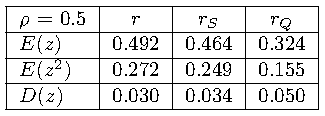
\includegraphics[]{LabSrcs/resources/20rho0.5.pdf}
    \end{center}
    \begin{center}
        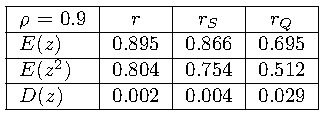
\includegraphics{LabSrcs/resources/20rho0.9.pdf}
    \end{center}
    \caption{Двумерное нормальное распределение, $n=20$}
    \label{tab:norm20}
\end{table}
\begin{table}[H]
    \begin{center}
    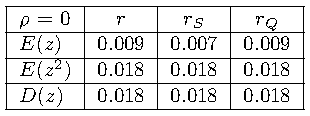
\includegraphics[]{LabSrcs/resources/60rho0.pdf}
    \end{center}
    \begin{center}
    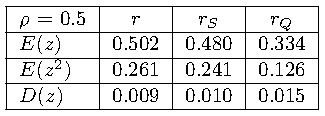
\includegraphics[]{LabSrcs/resources/60rho0.5.pdf}
    \end{center}
    \begin{center}
    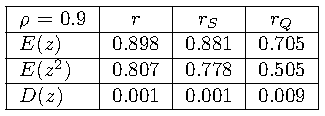
\includegraphics[]{LabSrcs/resources/60rho0.9.pdf}
    \end{center}
    \caption{Двумерное нормальное распределение, $n=60$}
    \label{tab:norm60}
\end{table}
\begin{table}[H]
    \begin{center}
    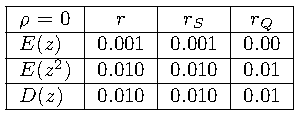
\includegraphics[]{LabSrcs/resources/100rho0.pdf}
    \end{center}
    \begin{center}
    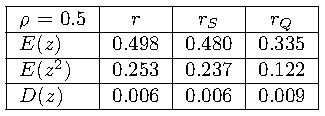
\includegraphics[]{LabSrcs/resources/100rho0.5.pdf}
    \end{center}
    \begin{center}
    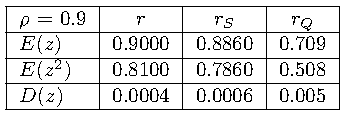
\includegraphics[]{LabSrcs/resources/100rho0.9.pdf}
    \end{center}
    \caption{Двумерное нормальное распределение, $n=100$}
    \label{tab:norm100}
\end{table}
\begin{table}[H]
    \begin{center}
    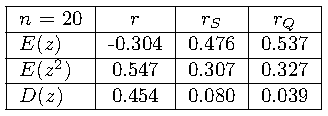
\includegraphics[]{LabSrcs/resources/mixedDistr20.pdf}
    \end{center}
    \begin{center}
    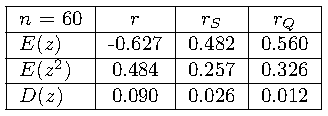
\includegraphics[]{LabSrcs/resources/mixedDistr60.pdf}
    \end{center}
    \begin{center}
    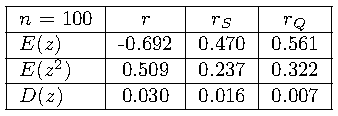
\includegraphics[]{LabSrcs/resources/mixedDistr100.pdf}
    \end{center}
    \caption{Смесь нормальных распределений}
    \label{tab:mixture}
\end{table}
\section{Обсуждение}
\section*{Примечание}
\begin{thebibliography}{9}
\bibitem{book1} 
 Максимов Ю.Д. Математика. Теория и практика по математической статистике. Конспект-справочник по теории вероятностей : учеб. пособие /
Ю.Д. Максимов; под ред. В.И. Антонова. $-$ СПб. : Изд-во Политехн.
ун-та, 2009. $-$ 395 с. (Математика в политехническом университете).
\end{thebibliography}
\end{document}
